\documentclass[landscape,final,paperwidth=36in,paperheight=24in,fontscale=0.55]{baposter}

\usepackage{calc}
\usepackage{graphicx}
\usepackage{amsmath}
\usepackage{amssymb}
\usepackage{relsize}
\usepackage{multirow}
\usepackage{rotating}
\usepackage{bm}

\usepackage{url}
\renewcommand{\thefootnote}{\roman{footnote}}	

\usepackage{pifont}% http://ctan.org/pkg/pifont
\newcommand{\cmark}{\ding{51}}%
\newcommand{\xmark}{\ding{55}}%

 \usepackage{enumitem}
   \setenumerate{nolistsep}
   \setitemize{nolistsep}

\def\labelitemi{\tiny$\blacksquare$}

\usepackage{graphicx}
\usepackage{multicol}

%\usepackage{times}
%\usepackage{helvet}
%\usepackage{bookman}
\usepackage{palatino}

\newcommand{\captionfont}{\footnotesize}

\renewcommand{\familydefault}{\sfdefault}

\graphicspath{{images/}{../images/}}
\usetikzlibrary{calc}

\newcommand{\SET}[1]  {\ensuremath{\mathcal{#1}}}
\newcommand{\MAT}[1]  {\ensuremath{\boldsymbol{#1}}}
\newcommand{\VEC}[1]  {\ensuremath{\boldsymbol{#1}}}
\newcommand{\Video}{\SET{V}}
\newcommand{\video}{\VEC{f}}
\newcommand{\track}{x}
\newcommand{\Track}{\SET T}
\newcommand{\LMs}{\SET L}
\newcommand{\lm}{l}
\newcommand{\PosE}{\SET P}
\newcommand{\posE}{\VEC p}
\newcommand{\negE}{\VEC n}
\newcommand{\NegE}{\SET N}
\newcommand{\Occluded}{\SET O}
\newcommand{\occluded}{o}
\newcommand{\specialcell}[2][c]{%
  \begin{tabular}[#1]{@{}c@{}}#2\end{tabular}}
%%%%%%%%%%%%%%%%%%%%%%%%%%%%%%%%%%%%%%%%%%%%%%%%%%%%%%%%%%%%%%%%%%%%%%%%%%%%%%%%
%%%% Some math symbols used in the text
%%%%%%%%%%%%%%%%%%%%%%%%%%%%%%%%%%%%%%%%%%%%%%%%%%%%%%%%%%%%%%%%%%%%%%%%%%%%%%%%

%%%%%%%%%%%%%%%%%%%%%%%%%%%%%%%%%%%%%%%%%%%%%%%%%%%%%%%%%%%%%%%%%%%%%%%%%%%%%%%%
% Multicol Settings
%%%%%%%%%%%%%%%%%%%%%%%%%%%%%%%%%%%%%%%%%%%%%%%%%%%%%%%%%%%%%%%%%%%%%%%%%%%%%%%%
\setlength{\columnsep}{1.5em}
\setlength{\columnseprule}{0mm}

%%%%%%%%%%%%%%%%%%%%%%%%%%%%%%%%%%%%%%%%%%%%%%%%%%%%%%%%%%%%%%%%%%%%%%%%%%%%%%%%
% Save space in lists. Use this after the opening of the list
%%%%%%%%%%%%%%%%%%%%%%%%%%%%%%%%%%%%%%%%%%%%%%%%%%%%%%%%%%%%%%%%%%%%%%%%%%%%%%%%
\newcommand{\compresslist}{%
\setlength{\itemsep}{1pt}%
\setlength{\parskip}{0pt}%
\setlength{\parsep}{0pt}%
}

%%%%%%%%%%%%%%%%%%%%%%%%%%%%%%%%%%%%%%%%%%%%%%%%%%%%%%%%%%%%%%%%%%%%%%%%%%%%%%
%%% Begin of Document
%%%%%%%%%%%%%%%%%%%%%%%%%%%%%%%%%%%%%%%%%%%%%%%%%%%%%%%%%%%%%%%%%%%%%%%%%%%%%%

\begin{document}

%%%%%%%%%%%%%%%%%%%%%%%%%%%%%%%%%%%%%%%%%%%%%%%%%%%%%%%%%%%%%%%%%%%%%%%%%%%%%%
%%% Here starts the poster
%%%---------------------------------------------------------------------------
%%% Format it to your taste with the options
%%%%%%%%%%%%%%%%%%%%%%%%%%%%%%%%%%%%%%%%%%%%%%%%%%%%%%%%%%%%%%%%%%%%%%%%%%%%%%
% Define some colors

%\definecolor{lightblue}{cmyk}{0.83,0.24,0,0.12}
\definecolor{lightblue}{rgb}{0.145,0.6666,1}

% Draw a video
\newlength{\FSZ}
\newcommand{\drawvideo}[3]{% [0 0.25 0.5 0.75 1 1.25 1.5]
   \noindent\pgfmathsetlength{\FSZ}{\linewidth/#2}
   \begin{tikzpicture}[outer sep=0pt,inner sep=0pt,x=\FSZ,y=\FSZ]
   \draw[color=lightblue!50!black] (0,0) node[outer sep=0pt,inner sep=0pt,text width=\linewidth,minimum height=0] (video) {\noindent#3};
   \path [fill=lightblue!50!black,line width=0pt] 
     (video.north west) rectangle ([yshift=\FSZ] video.north east) 
    \foreach \x in {1,2,...,#2} {
      {[rounded corners=0.6] ($(video.north west)+(-0.7,0.8)+(\x,0)$) rectangle +(0.4,-0.6)}
    }
;
   \path [fill=lightblue!50!black,line width=0pt] 
     ([yshift=-1\FSZ] video.south west) rectangle (video.south east) 
    \foreach \x in {1,2,...,#2} {
      {[rounded corners=0.6] ($(video.south west)+(-0.7,-0.2)+(\x,0)$) rectangle +(0.4,-0.6)}
    }
;
   \foreach \x in {1,...,#1} {
     \draw[color=lightblue!50!black] ([xshift=\x\linewidth/#1] video.north west) -- ([xshift=\x\linewidth/#1] video.south west);
   }
   \foreach \x in {0,#1} {
     \draw[color=lightblue!50!black] ([xshift=\x\linewidth/#1,yshift=1\FSZ] video.north west) -- ([xshift=\x\linewidth/#1,yshift=-1\FSZ] video.south west);
   }
   \end{tikzpicture}
}

\hyphenation{resolution occlusions}
%%
\begin{poster}%
  % Poster Options
  {
  % Show grid to help with alignment
  grid=false,
  columns=6,
  % Column spacing
  colspacing=1em,
  % Color style
  bgColorOne=white,
  bgColorTwo=white,
  borderColor=lightblue,
  headerColorOne=black,
  headerColorTwo=lightblue,
  headerFontColor=white,
  boxColorOne=white,
  boxColorTwo=lightblue,
  % Format of textbox
  textborder=roundedleft,
  % Format of text header
  eyecatcher=true,
  headerborder=closed,
  headerheight=0.1\textheight,
%  textfont=\sc, An example of changing the text font
  headershape=roundedright,
  headershade=shadelr,
  headerfont=\Large\bf\textsc, %Sans Serif
  textfont={\setlength{\parindent}{1.5em}},
  boxshade=plain,
%  background=shade-tb,
  background=plain,
  linewidth=2pt
  }
  % Eye Catcher
  {
\includegraphics[height=5em]{images/cornelltech.png}} 
  % Title
  {\bf\textsc{Weather Severity Prediction}\vspace{0.1em}}
  % Authors
  {\textsc{Alex Kopp, Andrew Li}\\ \vspace{0.5em}\textsc{\textbf{Mentors:} Serge Belongie, Alice Bonhomme-Biais}}
  % University logoWikipedia
  {% The makebox allows the title to flow into the logo, this is a hack because of the L shaped logo.
    
\includegraphics[height=6em]{images/google.jpg}
  }

%%%%%%%%%%%%%%%%%%%%%%%%%%%%%%%%%%%%%%%%%%%%%%%%%%%%%%%%%%%%%%%%%%%%%%%%%%%%%%
%%% Now define the boxes that make up the poster
%%%---------------------------------------------------------------------------
%%% Each box has a name and can be placed absolutely or relatively.
%%% The only inconvenience is that you can only specify a relative position 
%%% towards an already declared box. So if you have a box attached to the 
%%% bottom, one to the top and a third one which should be in between, you 
%%% have to specify the top and bottom boxes before you specify the middle 
%%% box.
%%%%%%%%%%%%%%%%%%%%%%%%%%%%%%%%%%%%%%%%%%%%%%%%%%%%%%%%%%%%%%%%%%%%%%%%%%%%%%
    %
    % A coloured circle useful as a bullet with an adjustably strong filling
    \newcommand{\colouredcircle}{%
      \tikz{\useasboundingbox (-0.2em,-0.32em) rectangle(0.2em,0.32em); \draw[draw=black,fill=lightblue,line width=0.03em] (0,0) circle(0.18em);}}

%%%%%%%%%%%%%%%%%%%%%%%%%%%%%%%%%%%%%%%%%%%%%%%%%%%%%%%%%%%%%%%%%%%%%%%%%%%%%%
  \headerbox{Opportunity/Value}{name=overview,column=0,row=0, span=3}{
%%%%%%%%%%%%%%%%%%%%%%%%%%%%%%%%%%%%%%%%%%%%%%%%%%%%%%%%%%%%%%%%%%%%%%%%%%%%%%
   \section*{Opportunity}
   \vspace{-3mm} 
   \indent \indent The National Weather Service (NWS) issues weather alerts in the event of an upcoming severe weather event. These alerts trigger systems that launch news, internet, and mobile messages to warn the public of threats to life and property. These alerts, however, do
not have a structured measure to indicate the actual severity of the weather event. As a result, a storm that passes by and causes little or no damage may have had the same Severe Thunderstorm Warning as the 2012 derecho that killed 22 people across seven states and left 4.2 million without power for an extended period. We were taked with building a model that can predict the severity of an upcoming storm based on the free-text descriptions and instructions inside the public alerts.

\textbf{Value Here}\\
test\\
test\\
test\\

 }


  
  %%%%%%%%%%%%%%%%%%%%%%%%%%%%%%%%%%%%%%%%%%%%%%%%%%%%%%%%%%%%%%%%%%%%%%%%%%%%%%
  \headerbox{Glossary}{name=glossary,column=3, span=3, row=0}{
%%%%%%%%%%%%%%%%%%%%%%%%%%%%%%%%%%%%%%%%%%%%%%%%%%%%%%%%%%%%%%%%%%%%%%%%%%%%%%
   \vspace{0.3em}
   \begin{multicols*}{2}
	\setlength\multicolsep{0pt}
   \begin{description}
   \setlength{\itemsep}{1pt}
   \setlength{\itemindent}{-1em}
   \setlength{\leftmargin}{-23em}
   \item[NWS] National Weather Service
   \item[NOAA] National Oceanic and Atmospheric Administration
   \item[CAP] Common Alerting Protocol. The protocol used by the National Weather Service to send out weather alerts.
   \item[Storm Event Database] A database of storm damage, injuries, and deaths managed by the National Oceanic and Atmospheric Administration
   \item[Tokenizing] Breaking a string of text into meaningful sections (tokens). For this project, we broke text into words.
   \item[Stemming] Reducing words to their root form. For example: "educate" and "educational" both get reduced to "educ"
   \item[TFIDF] Term frequency-inverse document frequency. A term weighting method that uses both the frequency of the term in the document as well as the frequency of the term across the rest of the corpus
   \item[Stop Words] Extremely common words that add little to no value to a sentence
   \item[N-Grams] Sequences of words of length $N$
   \end{description}
   \end{multicols*}
 }
 %%%%%%%%%%%%%%%%%%%%%%%%%%%%%%%%%%%%%%%%%%%%%%%%%%%%%%%%%%%%%
  
  %%%%%%%%%%%%%%%%%%%%%%%%%%%%%%%%%%%%%%%%%%%%%%%%%%%%%%%%%%%%%%%%%%%%%%%%%%%%%%
  \headerbox{Results}{name=results,column=3, span=3, row=0, below=glossary}{
%%%%%%%%%%%%%%%%%%%%%%%%%%%%%%%%%%%%%%%%%%%%%%%%%%%%%%%%%%%%%%%%%%%%%%%%%%%%%%
  \begin{center}
  %\includegraphics[width=1\linewidth]{images/diagram.pdf}
  \begin{tabular}{r|cccccc}
  & \textbf{Property Damage} & \textbf{Crop Damage} & \textbf{Direct Deaths} & \textbf{Indirect Deaths} & \textbf{Direct Injuries} & \textbf{Indirect Injuries} \\ 
\hline 
\rule{0pt}{2ex} \textbf{Classification Accuracy} & $88\%$ & $98.77\%$ & $99.5\%$ & $99.94\%$ & $99.4\%$ & $99.91\%$ \\ 
\textbf{Base Rate}                               & $24.36\%$ & $2.2\%$ & $0.5\%$ & $0.06\%$ & $0.6\%$ & $0.09\%$ \\ 
\hline
\hline
\textbf{Improvement} & $\color{green} 12.36\%$ & $\color{orange} 0.97\%$ & $\color{red} 0.00\%$ & $\color{red} 0.00\%$ & $\color{red} 0.00\%$ & $\color{red} 0.00\%$ \\ 
\end{tabular} \\
\textit{Classification - Predicting whether a NWS CAP report will lead to at least \textbf{one} of each respective storm severity indicator}\\
\textit{Base Rate - The percentage of NWS CAP reports in our database that have at least \textit{one} of each respective storm severity indicator}
  \end{center}

  \begin{center}
  
   %\includegraphics[width=0.8\linewidth]{images/fixedCgraph.pdf}
\begin{tabular}{r|ccccc}
%& \multicolumn{5}{c}{\textbf{Algorithm}} \\
 & \textbf{Property Damage} & \textbf{Crop Damage} \\ 
\hline 
$\boldsymbol R^2$ & $\color{red} -0.00138520002963$ \footnote{Yes, an $R^2$ value can be negative} & $\color{orange} 0.389844743554$ \\ 
\textbf{Regression} & Stochastic Gradient Descent Regressor & Stochastic Gradient Descent Regressor &  &  &  \\ 
\textbf{Loss Function} & Huber & Squared Loss \\ 
\textbf{Penalty} & L2 & L1 \\ 
\textbf{Iterations} & $300$  & $300$ \\ 
\end{tabular} 

\end{center}

   \vspace{0.3em}
 }
 %%%%%%%%%%%%%%%%%%%%%%%%%%%%%%%%%%%%%%%%%%%%%%%%%%%%%%%%%%%%%

%%%%%%%%%%%%%%%%%%%%%%%%%%%%%%%%%%%%%%%%%%%%%%%%%%%%%%%%%%%%%%%%%%%%%%%%%%%%%%
\headerbox{Discussion}{name=discussion,column=3,span=3,row=0, below=results}{
  %%%%%%%%%%%%%%%%%%%%%%%%%%%%%%%%%%%%%%%%%%%%%%%%%%%%%%%%%%%%%%%%%%%%%%%%%%%%%%
  
\begin{itemize}
 \setlength{\itemindent}{-1em}
\item \textbf{Results} - Test T
\item \textbf{Matching storms across data sets takes creativity and error prone} - Test T
\item \textbf{Predicting casualties turned out to be more difficult than expected} - Test T
\item \textbf{Large amounts of sparse data can be difficult to work with} - Test
\end{itemize}

}


%%%%%%%%%%%%%%%%%%%%%%%%%%%%%%%%%%%%%%%%%%%%%%%%%%%%%%%%%%%%%%%%%%%%%%%%%%%%%%
\headerbox{Next Steps}{name=nextsteps,column=3,span=3,row=0,below=discussion, above=bottom}{
  %%%%%%%%%%%%%%%%%%%%%%%%%%%%%%%%%%%%%%%%%%%%%%%%%%%%%%%%%%%%%%%%%%%%%%%%%%%%%%

\begin{itemize}
 \setlength{\itemindent}{-1em}
\item \textbf{Acquire more NWS CAP reports and NOAA Storm Event Database entries} - Test T
\item \textbf{Additional domain knowledge} - Test T
\item \textbf{Build additional models from different data sets} - Test
\end{itemize}

   \vspace{0.0em}
}
%%%%%%%%%%%%%%%%%%%%%%%%%%%%%%%%%%%%%%%%%%%%%%%%%%%%%%%%%%%%%%%%%%%%%%%%%%%%%%
  \headerbox{Method}{name=method,column=0,below=overview, span=3, bottomaligned=nextsteps}{
%%%%%%%%%%%%%%%%%%%%%%%%%%%%%%%%%%%%%%%%%%%%%%%%%%%%%%%%%%%%%%%%%%%%%%%%%%%%%%
\textbf{Approach} Since we were not given a precise definition of "severity," it was left to us to determine which factors govern the severity of a storm. Since we only had access to \textit{direct deaths}, \textit{indirect deaths}, \textit{direct injuries}, \textit{indirect injuries}, \textit{property damage}, and \textit{crop damage}, we transformed the task into building a model to predict each of these severity indicators.\\

\noindent{\centering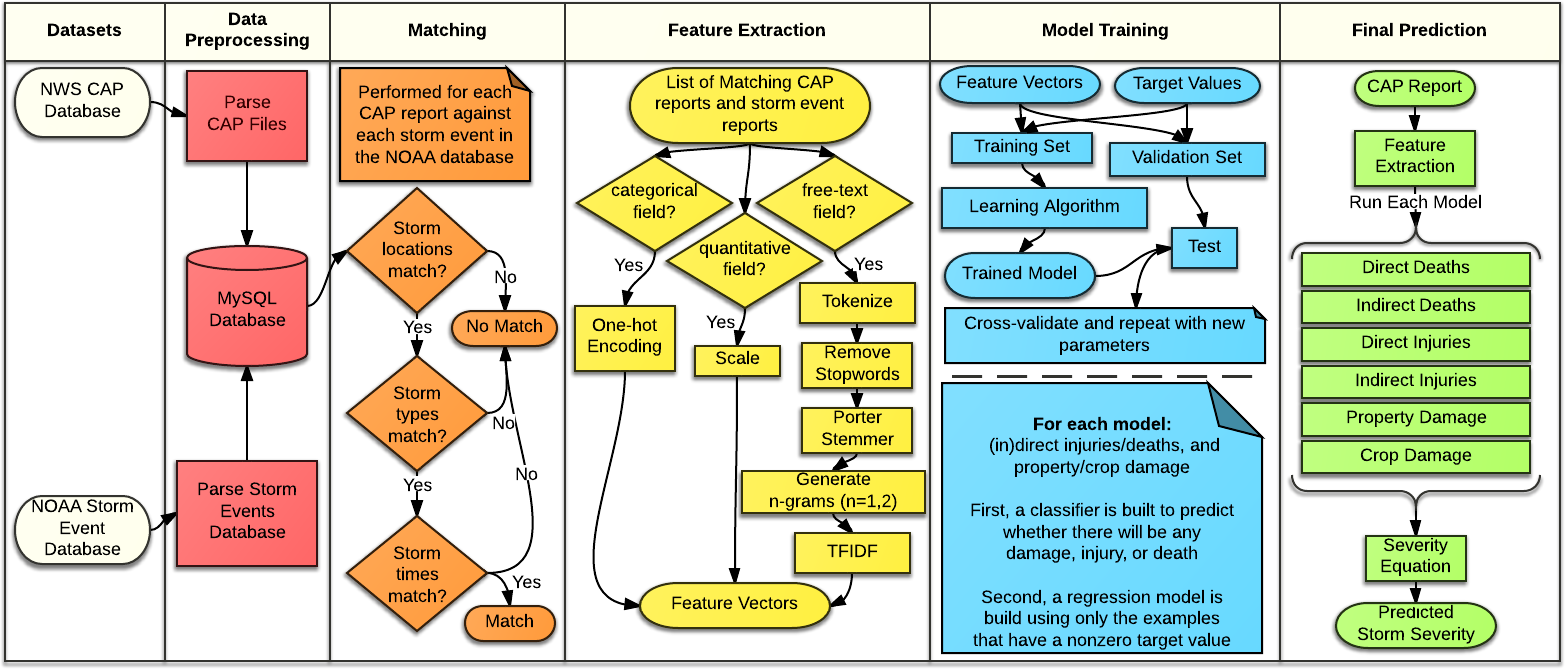
\includegraphics[width=0.75\linewidth]{images/Method.png}\\}
\begin{multicols*}{2}
	\setlength\multicolsep{0pt}
	\begin{enumerate}
	   \setlength{\itemindent}{-1em}
		\setlength{\itemsep}{3pt}
		\item \textbf{Data Preprocessing} 
		\begin{enumerate}[leftmargin=2em]
			\setlength{\itemindent}{-1.5em}
			\item \textbf{Parsing CAP Reports} - Used NWS CAP Parser package for Python. Converted dates/times to UTC. Assumed a storm's start date/time was given by the \textit{onset} attribute in the CAP report. If that attribute was not populated, the \textit{effective} attribute was used. If the \textit{effective} attribute was not populated, the mandatory \textit{sent} field was used.
			\item \textbf{Parsing NOAA Storm Events Database} - Used Python's CSV parsing package. Unfortunately, the CSV is malformed (quotes and commas are present and not escaped in free-text fields). Luckily, the malformed portion comes after the information that was needed. Converted dates/times to UTC. Converted \textit{property damage} and \textit{crop damage} fields from shorthand notation to an actual number (e.g $100K \rightarrow 100000$)
		\end{enumerate}

		\item \textbf{Matching}
		\begin{enumerate}[leftmargin=2em]
			\setlength{\itemindent}{-1.5em}
			\item \textbf{Location Matching} - Used the \textit{FIPS 6-4} attribute in both CAP report and Storm Event Database to link counties and states.
			\item \textbf{Storm Type Matching} - Since the NWS and NOAA have differing storm types, a matching process had to be done associating one agency's storm types to the other. With the help of Alice Bonhomme-Biais, a list of plausible event type matches was constructed.
			\item \textbf{Time Matching} - To account for minor differences in time between the data sets, a particular CAP report must overlap an entry in the Storm Event Database by at least $25\%$ to be considered a match
		\end{enumerate}

		\item \textbf{Feature Extraction} - The process of extracting features creates a vector representation of each example in our data sets. More concretely, each NWS CAP report needs to be converted into a vector of numbers. A CAP report has three types of data in it: categorical, quantitative, and free text. For categorical data, we used a one-hot encoding representation. For quantitative fields, we scaled the values using scikit-learn's \textit{StandardScaler}. Finally, free text fields were processed in the following steps:
		\textbf{Tokenization}, \textbf{Stopword Removal}, \textbf{Porter Stemming}, \textbf{Unigram and Bigram Generator}, and \textbf{TFIDF Weighting}
		
		Ultimately, we had $457,351$ features for each of the $202,856$ examples in the data set.

		\item \textbf{Model Training} - Since we are trying to predict real, continuous numbers, a regression algorithm is the tool for the job. Since the majority of training examples have zero injuries/deaths/damage, we actually built a classifier in addition to a regressor. The classifier would predict whether or not there would be \textit{any} injuries/deaths/damage. The logic behind this is to only use the regression model if the classifier gives a positive result. Our results are displayed in the Results section.

		\item \textbf{Final Prediction} - Although this step is incomplete, it is pretty trivial to create once satisfactory models are built. At a high level, a new CAP report is converted into a vector in the same way that the feature extraction was performed on the training data. Next, the vector is passed into each of the injury/death/damage models. A real number is returned. Then, the predicted values get plugged into an equation to transform into a categorical storm severity value.
	 \end{enumerate}
 \end{multicols*}
  }
%%%%%%%%%%%%%%%%%%%%%%%%%%%%%%%%%%%%%%%%%%%%%%%%%%%%%%%%%%%%%%%%%%%%%%%%%%%%%%


\end{poster}

\end{document}
